% *******************************************************************************
% * Copyright (c) 2007 by Elexis
% * All rights reserved. This document and the accompanying materials
% * are made available under the terms of the Eclipse Public License v1.0
% * which accompanies this distribution, and is available at
% * http://www.eclipse.org/legal/epl-v10.html
% *
% * Contributors:
% *    G. Weirich
% *
% *  $Id: elexis-nachrichten.tex 4878 2008-12-30 13:51:18Z rgw_ch $
% *******************************************************************************

\documentclass[a4paper]{scrartcl}
\usepackage{german}
\usepackage[utf8]{inputenc}
\usepackage{makeidx}
\makeindex
% Hier ein etwas skurriler Block, der dazu dient, die Unterschiede
% zwischen pdflatex und latex auszubügeln
% Grafiken müssen als png oder gif (für pdflatex) und als eps (für Latex)
% vorhanden sein. Die Endung kann man beim \includegraphics jeweils weglassen,
% das System nimmt je nach Renderer die geeignete Variante.

\usepackage[pdftex]{graphicx}
\DeclareGraphicsExtensions{.pdf,.jpg,.png}

\usepackage{floatflt}
\usepackage{wrapfig}
\usepackage[]{hyperref}
\usepackage{color}
\begin{document}
\title{Elexis-Nachrichten-Plugin}
\author{Gerry Weirich}
\maketitle

\section{Einführung}
Dieses Plugin ermöglicht eine einfache Nachrichtenübermittlung zwischen verschiedenen Mitarbeitern. Im Gegensatz zu Remindern erscheinen diese Nachrichten immer als Dialogbox.

\subsection{Nachricht erstellen}
\begin{wrapfigure}{r}{2cm}
    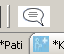
\includegraphics{newmsg}
\end{wrapfigure}

\bigskip

Wenn das Plugin installiert ist, erscheint in der Haupt-Werkzeugleiste von Elexis der Knopf 'Nachricht erstellen' (s. Bild). Klick auf dieses Werkzeug öffnet den Dialog 'Nachricht erstellen':

\begin{figure}[htp!]
    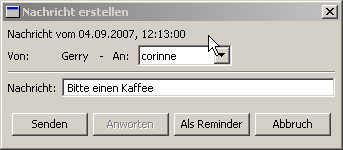
\includegraphics{newmsg2}
    \caption{Neue Nachricht erstellen}
\end{figure}

Mit Klick auf 'senden' wird die Nachricht abgesendet. Elexis findet automatisch die Arbeitsstation, auf der die Empfängerin eingeloggt ist und zeigt dort die Nachricht an. Wenn der Empfänger zur Zeit nicht eingeloggt ist, erscheint die Nachjricht sofort beim nächsten Einloggen. Wenn sie an mehreren Arbeitsstationen eingeloggt ist, erscheint die Nachricht auf allen.

\bigskip

\begin{figure}[htp]
    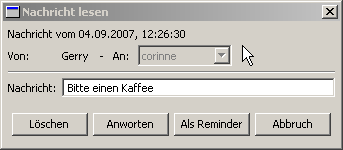
\includegraphics{newmsg3}
    \caption{Nachricht lesen}
\end{figure}

Die Empfängerin hat folgende Möglichkeiten:
\begin{itemize}
\item Löschen - Nachricht wird gelöscht und erscheint nicht mehr
\item Antworten - Es wird eine Nachricht an den Absender erstellt. Die ursrünglich Nachricht wird gelöscht.
\item Als Reminder - Die Nachricht wird in einen Reminder umgewandelt und bleibt so erhalten
\item Abbruch - Die Anzeige wird geschlossen, abe die Nachricht erscheint nach einiger Zeit erneut.
\end{itemize}

\bigskip

\textbf{Konfiguration}
Es ist keine Spezielle Konfiguration notwendig. Der Zeitabstand zwischen Absenden und Erscheinen der Nachricht hängt vom 'Heartbeat' ab (Datei-Einstellungen-Allgemein-Aktualisierungsintervall)

\end{document} 